% Deployment view subsection, to be included in architecture.tex

\subsection{Deployment view}
\label{sect:deploy}
The deployment view of the application can be seen in Figure \ref{deploy}. 
It uses a 5-tier architecture to separate the web aspects from the application itself and from the data. This way, the code can be better decomposed to increase reusability and for security reasons, exposing only the web tier to browsers. The safety of the system is ensured by the use of two DMZs, one isolating the web tier from the rest and one to better protect the data layer. 

With respect to the theoretical layer subdivision, layers 2 and 3 have been united through the use of Apache Tomcat, that covers both the web server's and servlet container's functions.

\begin{landscape}
	\begin{figure}[p]
		\centering	
		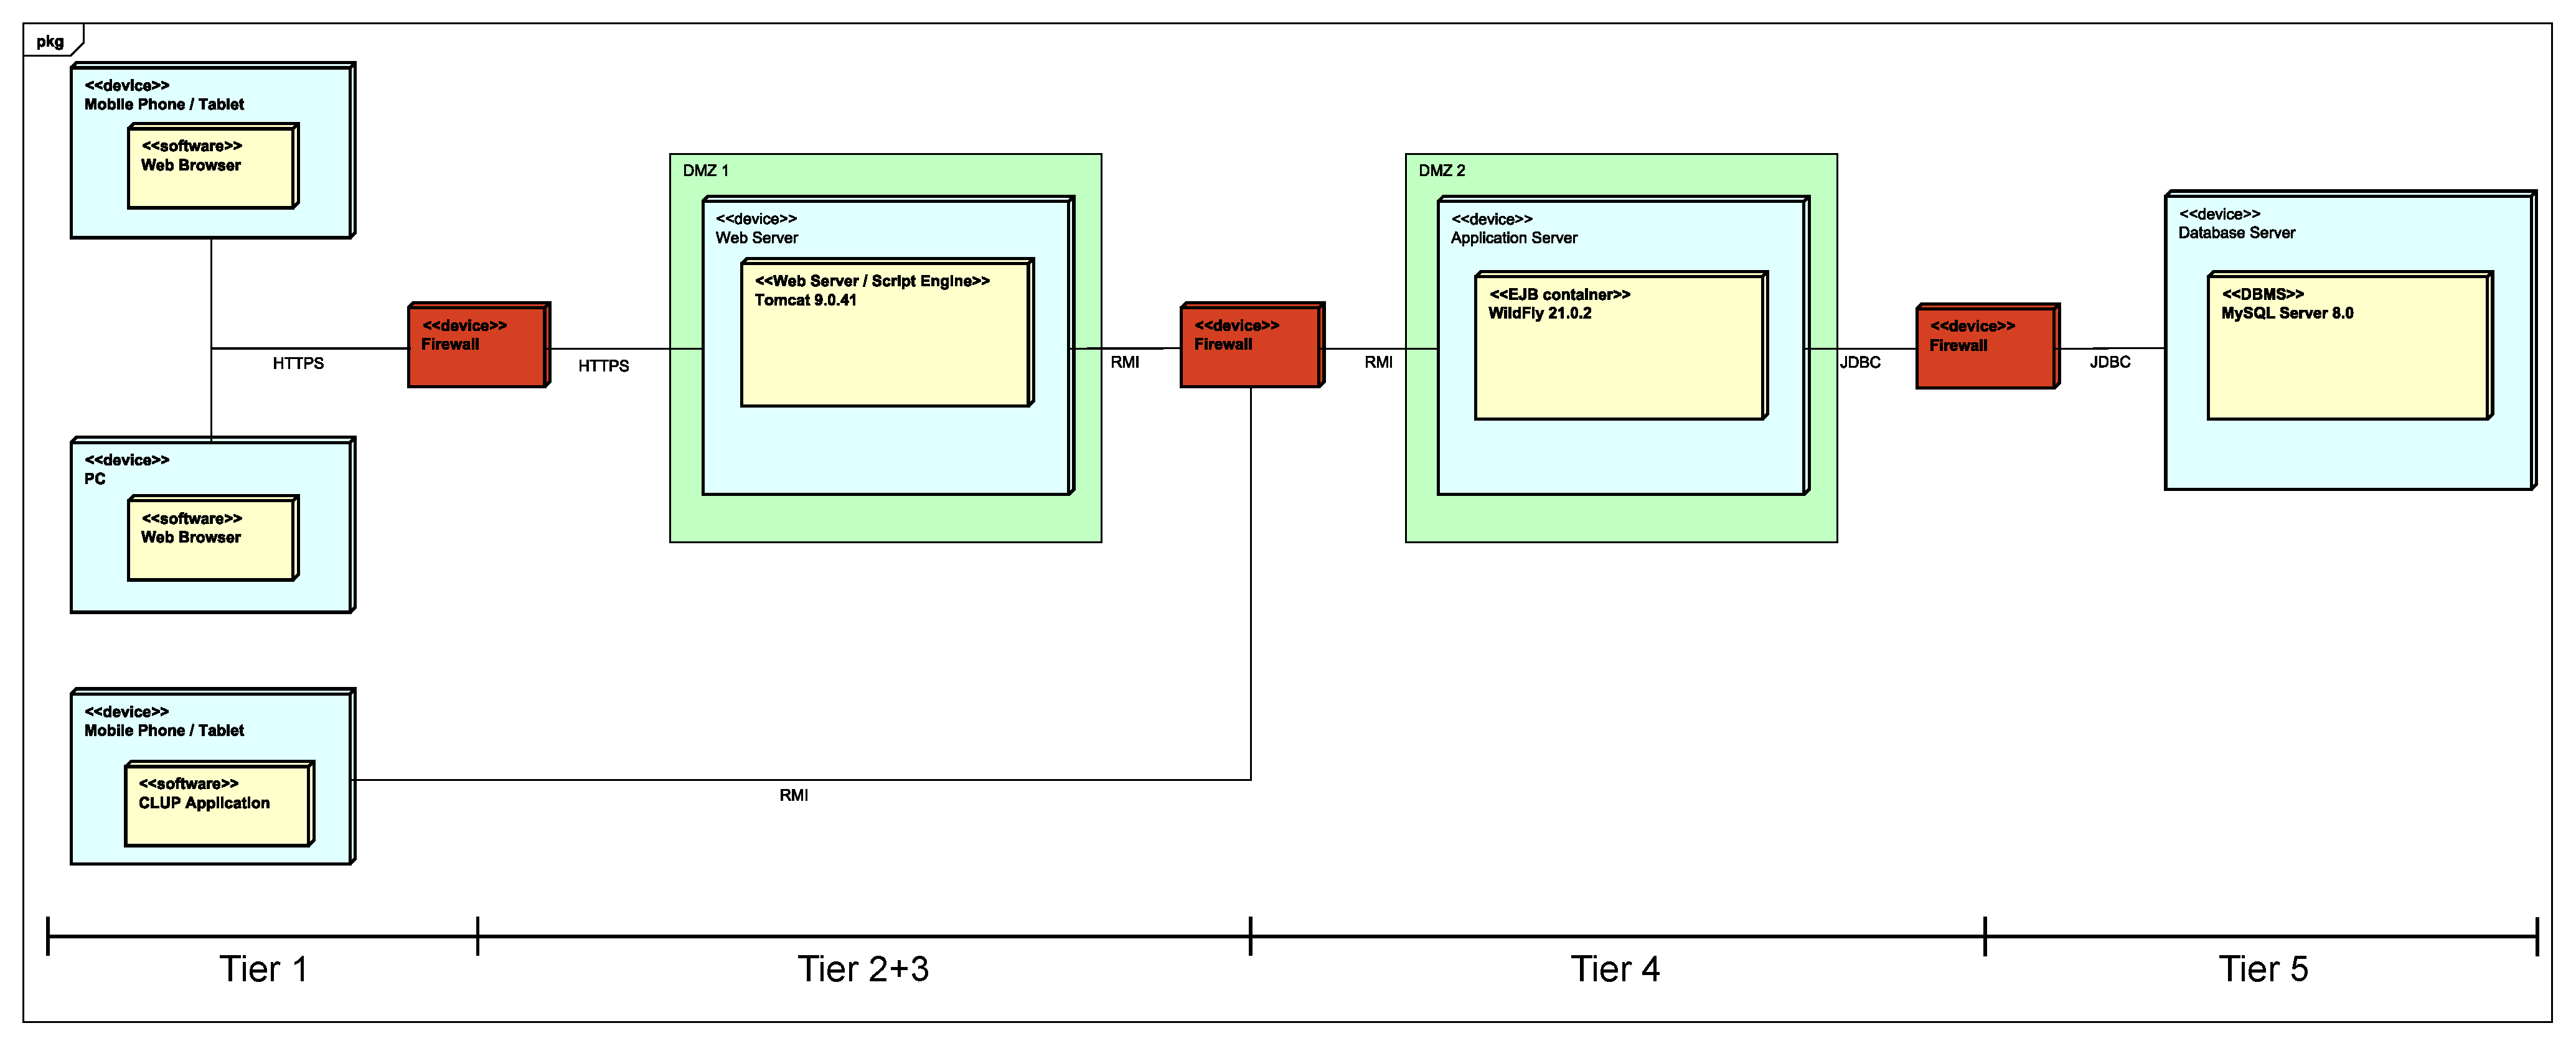
\includegraphics[width=\linewidth] {deployment_diagrams/deployment}
		\caption{Deployment diagram of the application}
		\label{deploy} 
	\end{figure}
\end{landscape}
